\documentclass{beamer}

% \usepackage{default}
\usepackage[ngerman]{babel} % Deutsche Formattierung
\usepackage[T1]{fontenc}
\usepackage[utf8]{inputenc} % Zeichenkodierung
\usepackage{color} % Farben
\usepackage{setspace} % Das Paket setspace ermöglicht ein einfaches Umstellen von normalem, anderthalbfachen oder doppeltem Zeilenabstand.
\usepackage{graphicx} % Bilder
\usepackage[final]{listings}  % ermöglicht die Darstellung von (Programm-)Quellcode in der Arbeit
\usepackage[normalem]{ulem} % ermöglicht das Unterstreichen von Text
\usepackage{amsfonts} % ok-zeichen usw
\usepackage{amsmath} % mathekrams
\usepackage{scrpage2}
\usepackage{babelbib} % Bibliographie
\usepackage{array} % für tabellen
\usepackage[style=base,margin=10pt,font=footnotesize,labelfont=bf]{caption} % Formattierung Bildunterschrift
\usepackage{listings} % Quellcode
\usepackage{float} % floating figures
\usepackage{tikz} % Diagramme
\usepackage{wrapfig} % Text neben Abbildungen
\usepackage{pdflscape} % Seiten in Querformat
\usepackage{geometry}
\usepackage{soul}
\usepackage{textcomp} % Quote Symbol
\usepackage{pifont}% http://ctan.org/pkg/pifont

\newcommand{\cmark}{\ding{51}}%
\newcommand{\xmark}{\ding{55}}%

\newcommand{\routput}{\vspace{-0.25cm}\hspace{5pt}\footnotesize\color{blue}\ttfamily} 
\newcommand{\rsymbol}{\vspace{-0.25cm}\hspace{5pt}\footnotesize\color{blue}\ttfamily\textquotesingle}
\newcommand{\rerror}{\vspace{-0.25cm}\hspace{5pt}\footnotesize\color{red}\ttfamily$\bigotimes$ \hspace{0cm}}

\newcommand{\q}{\textquotesingle}
\newcommand{\qq}{\textquotedbl}

\lstset{
    backgroundcolor=\color{white}, 		% white background
    %     columns=fullflexible, 			% allow latex to break lines
    numbers=none, 				% no line numbering
    showstringspaces=false, 			% no gap character in strings
    belowskip=-10pt, 				% remove blank space at the bottom of listing
    basicstyle=\ttfamily\footnotesize\color{darkblue}, 
    xleftmargin=5pt, % Padding
    language=Lisp, 				% for highliting comments and literals
    commentstyle=\color{beige}, 		% comment style
    stringstyle=\color{green}, 			% literal style
    numberstyle=\color{green},
    alsoletter={\#, >},
    keywordstyle=\ttfamily, 			% keyword style
    keywordstyle=[2]\color{green},		% style for literals
    keywordstyle=[3]\color{black},	% style for non-terminals
    literate=
	  *{(}{{{\color{brown}{(}}}}{1} 	% colored brackets
	  {)}{{{\color{brown}{)}}}}{1}	 	
	  {{[}}{{{\color{brown}{{[}}}}}{1}
	  {{]}}{{{\color{brown}{{]}}}}}{1}
	  {\{}{{{\color{brown}{\{}}}}{1}
	  {\}}{{{\color{brown}{\}}}}}{1}
	  {'}{{{\bfseries\color{green}{\textquotesingle}}}}{1}
	  {\#}{{{\color{green}{\#}}}}{1}
	  {`}{{{\textquoteleft}}}{1}
	  {lambda}{{$\lambda$}}{1},
%     % lists of keywords
%     morekeywords={},
    keywords=[2]{\#t, \#f},
    keywords=[3]{\#lang swindle, \#lang racket, >} 
}

\makeatletter
\newcommand{\thickhline}{%
    \noalign {\ifnum 0=`}\fi \hrule height 1.2pt
    \futurelet \reserved@a \@xhline
}
\newcolumntype{'}{@{\hskip\tabcolsep\vrule width 1.2pt\hskip\tabcolsep}}
\makeatother

\usetheme{Darmstadt}
\useoutertheme{tree}
\useinnertheme{rectangles}

% Farben
\definecolor{uhhred}{cmyk}{0,1,1,0}
\definecolor{beige}{RGB}{194,116,31}
\definecolor{green}{RGB}{41,128,38}
\definecolor{brown}{RGB}{132,60,36}
\definecolor{darkblue}{RGB}{38,38,128}
\definecolor{darkred}{RGB}{200,0,0}
\definecolor{darkgreen}{RGB}{0,150,0}
\definecolor{purple}{RGB}{100,0,100}
\definecolor{darkblue}{RGB}{0,0,128}
\definecolor{turquoise}{RGB}{95,158,160}

% Tikz styles
\usetikzlibrary{shapes,arrows,decorations.markings}
\tikzstyle{block} = [rectangle, draw, fill=gray!15, text width=11em, text centered, rounded corners, minimum height=3em]
\tikzstyle{label} = [text centered]
\tikzstyle{arrow} = [draw, -latex', thick, postaction={decorate}] 
\tikzstyle{line} = [draw, -, thick]

\institute[FBI - UniHH]{Universität Hamburg - Fachbereich Informatik}
\title{Untersuchungen zur Integration von CLOS-Konzepten in das Objektsystem von Racket}
\subtitle{Masterarbeit}
\author{Manuela Beckert}
\date{27. Juni 2017}

\begin{document}

\maketitle

\frame{\tableofcontents}


\section{Problemstellung}
\begin{frame}
\frametitle{Mehrfachvererbung -- Das Diamond-Problem}
 \begin{figure}
\centering
 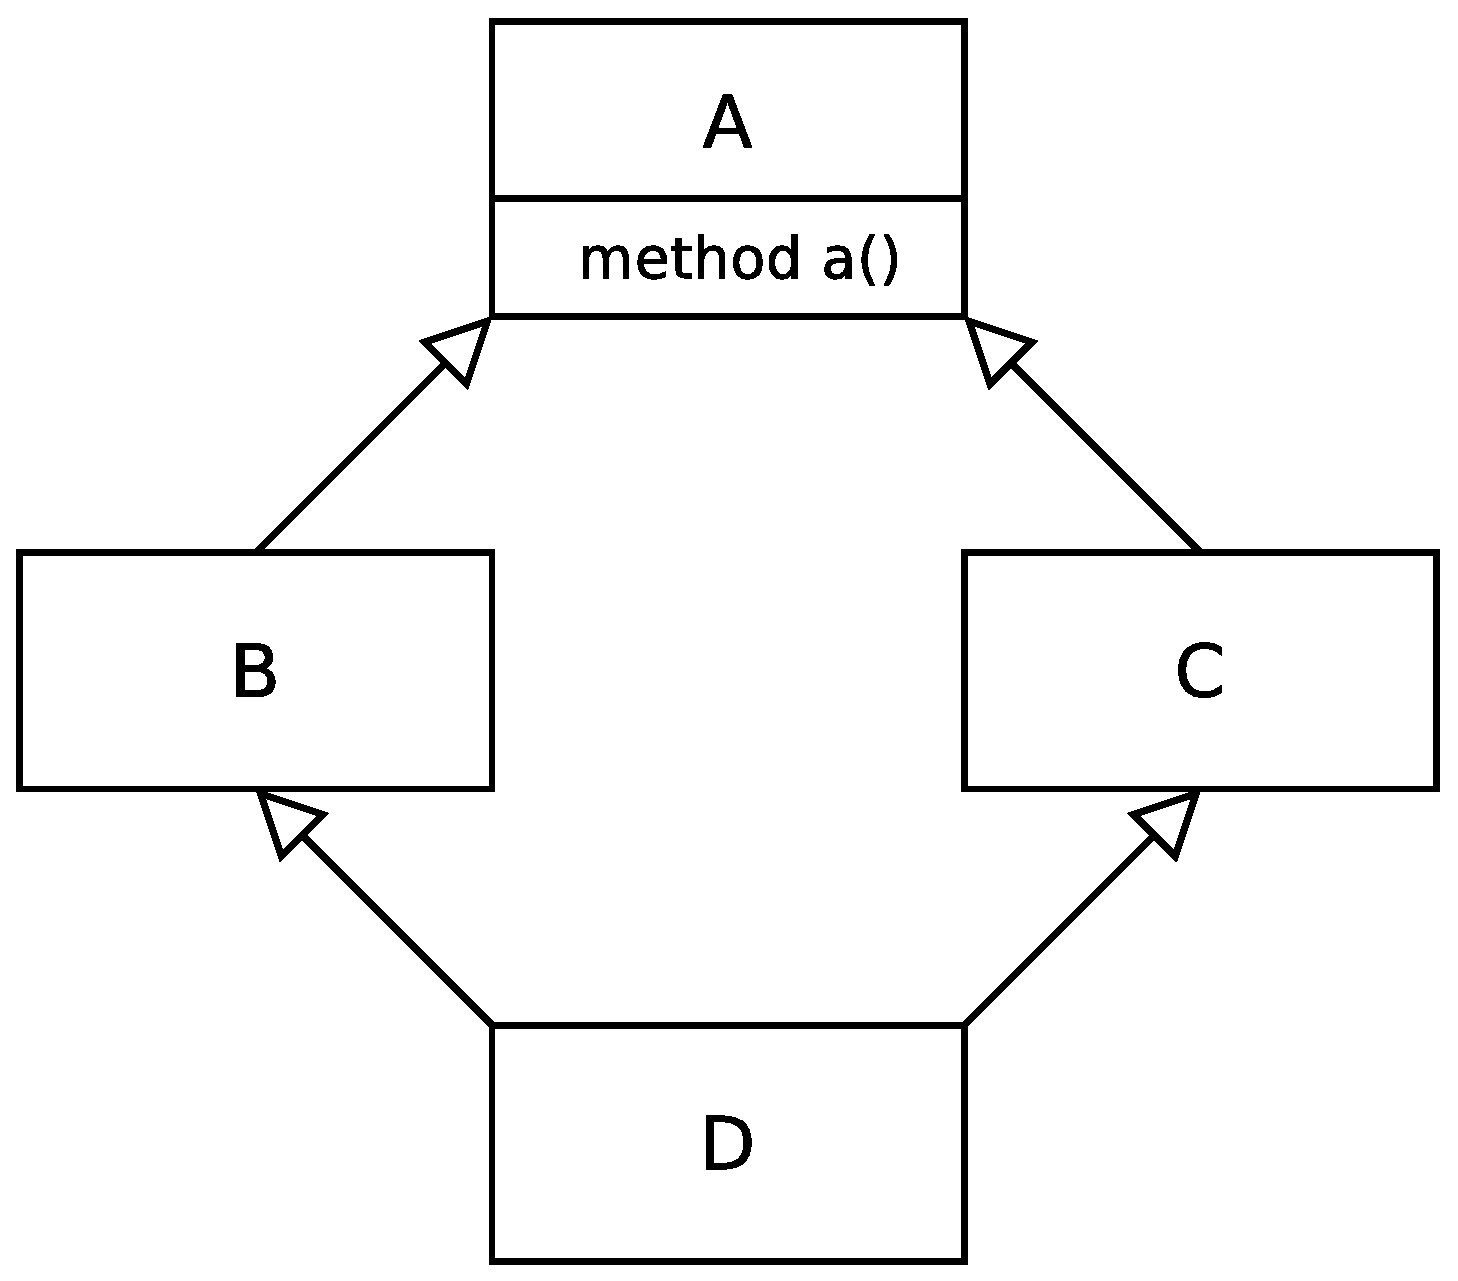
\includegraphics[scale = 0.27]{pictures/diamond}
 \caption{Das Diamond-Problem.}
\end{figure}
\end{frame}

\begin{frame}
 \frametitle{Herangehensweisen}
 \begin{columns}
  \begin{column}{0.7\textwidth}
   \begin{itemize}
    \item keine Unterstützung (Java $<$7\only<2>{, {\color{blue}Racket}})
    \item Fehler bei Verwendung mehrdeutiger Eigenschaften (Go, Java 8)
    \item Wahl der zu vererbenden Eigenschaften per Hand (Eiffel)
    \item Umbenennung gleichbenannter Eigenschaften (Eiffel, Longtalk)
    \item Qualifizierter Zugriff (C++, OCaml)
    \item Präzedenz (\only<1>{Common Lisp}\only<2>{{\color{blue}{Common Lisp}}}, Perl, Python)
    \item Kombination gleichbenannter Eigenschaften (\only<1>{Common Lisp}\only<2>{{\color{blue}{Common Lisp}}}, Eiffel)
   \end{itemize}
  \end{column}
 \begin{column}{0.3\textwidth}
  \begin{figure}[h]
   \centering
   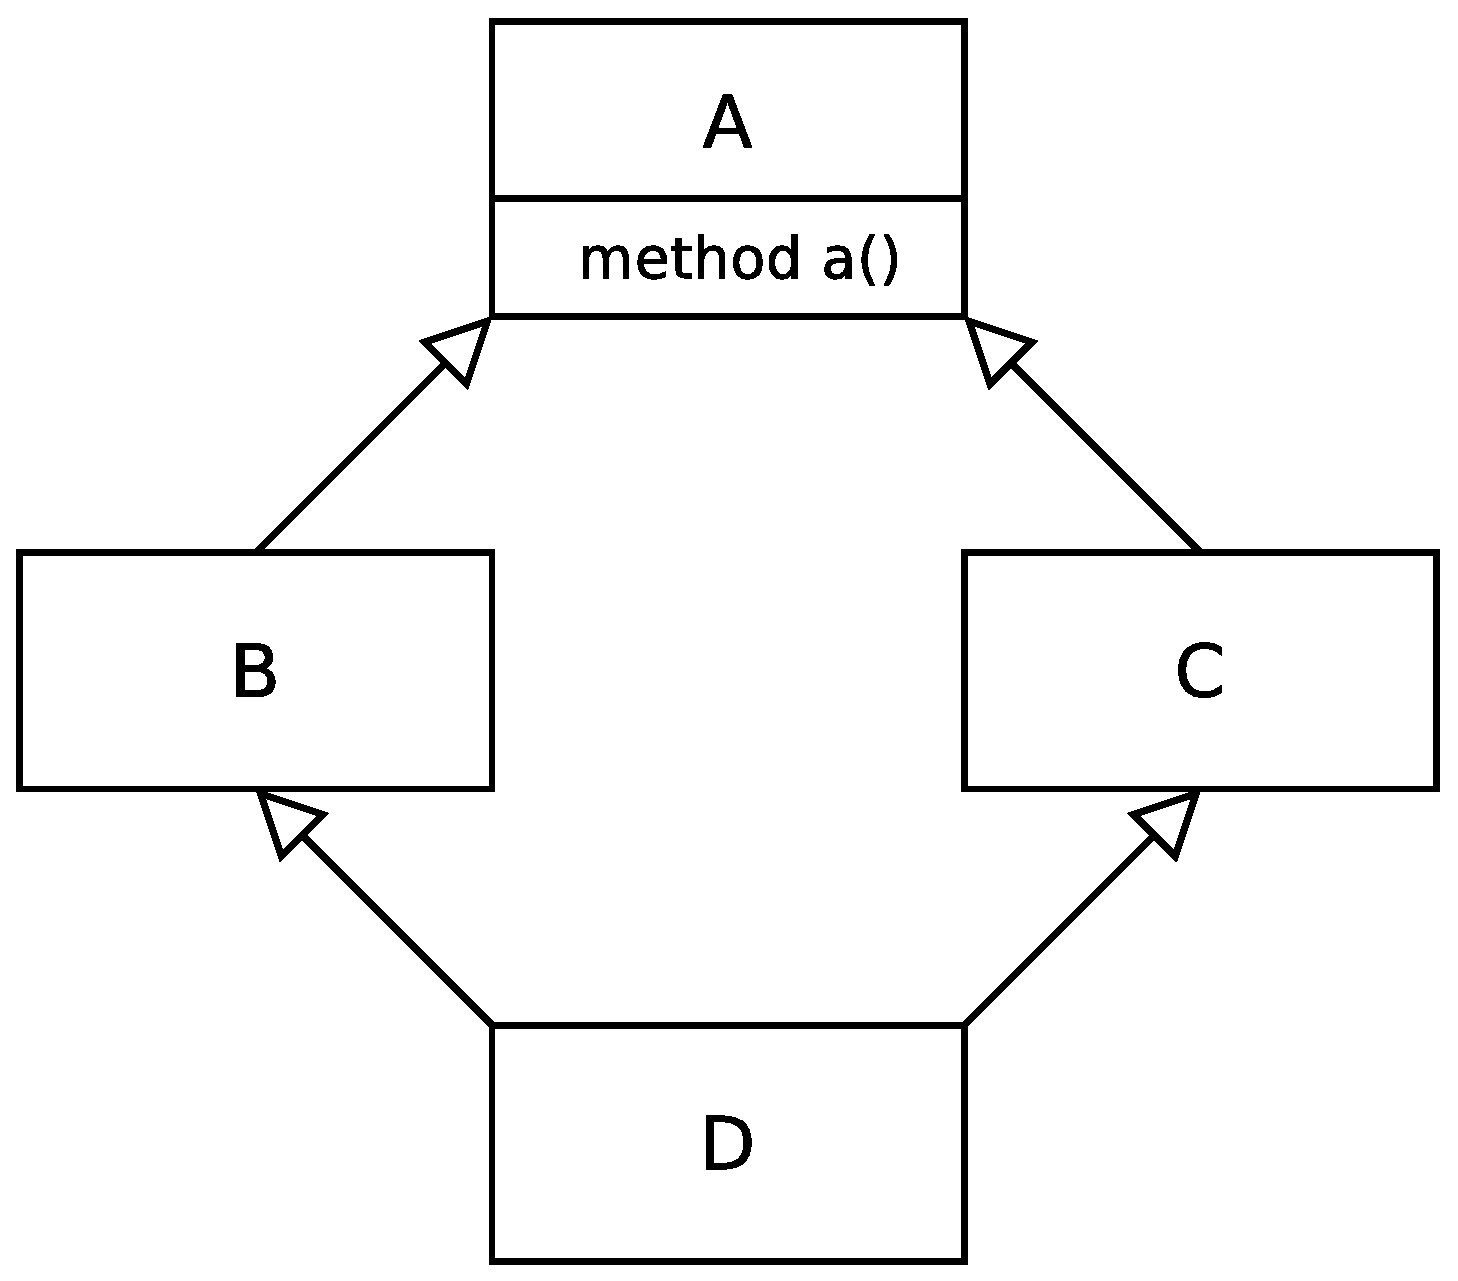
\includegraphics[scale = 0.15]{pictures/diamond}
  \end{figure}
 \end{column}
 \end{columns}
\end{frame}

\begin{frame}
 \frametitle{Problemstellung}
 Ziel: Mehrfachvererbung im Objektsystem von Racket
 \vspace{0.5cm}
 \begin{itemize}
  \item CLOS bietet sehr einstiegsfreundliche Implementation
  \item Implementierung von CLOS in Racket existiert
  \item[\textbf{\textrightarrow}] Features von CLOS in Racket integrieren
 \end{itemize}
 \vspace{0.2cm}
 \begin{itemize}
  \item wenig Forschung zum Thema 
  \item Implementation von CLOS nutzt ein Metaobjektprotokoll
  \item Informationen über Klassen und Objekte in internen Objekten
  \item[\textbf{\textrightarrow}] Untersuchen, ob Metaobjektprotokoll auch zur Erweiterung von Racket genutzt werden kann
  \item[\textbf{\textrightarrow}] Spracherweiterung, u.a. für die Lehre
 \end{itemize}
\end{frame}

\section{Objektsysteme in Racket}
\subsection{Das Objektsystem von Racket}
\frame{\tableofcontents[currentsection, currentsubsection]}

\begin{frame}
 \frametitle{Ein Beispiel für Mehrfachvererbung}
 \begin{figure}
 \centering
 \includegraphics[scale=0.27]{pictures/pokemon}
 \caption{Vererbungshierarchie für die Klasse Pokemon.}
 \end{figure}
\end{frame}

\begin{frame}[fragile]
 \frametitle{Einfache Klassen}
 \begin{lstlisting}
(define Thing 
  (class object% (super-new)
    (init-field [name "a Thing"])
    (define/public (who-are-you?) 
      (string-append "I am " name "!"))))
 \end{lstlisting}
\end{frame}

\begin{frame}[fragile]
 \frametitle{Vererbung}
 \begin{lstlisting}
(define Element 
  (class Thing (super-new)
    (init-field [attr 'water])))
    
(define Animal 
  (class Thing
    (init-field [size 'small])))
    
    
> (send (new Element [name "Fire"] [attr 'fire]) 
        who-are-you?)
\end{lstlisting} \vspace{0.6cm}
{\routput {\qq}I am Fire!\qq}\\
\vspace{0.5cm}
\begin{itemize}
 \item Es gib Mixins und Traits
 \item aber: beides geschickt verpackte Einfachvererbung
\end{itemize}
\end{frame}

\begin{frame}
 \frametitle{Ergänzungsmethoden}
\begin{table}
 \centering \small
\begin{tabular}{|c'c|c|c|c|c}
 \hline
		& \multicolumn{1}{p{1.6cm}|}{\centering\footnotesize überschreibt geerbte Methode} 
		& \multicolumn{1}{p{1.6cm}|}{\centering\footnotesize erweitert geerbte Methode}
		& \multicolumn{1}{p{1.6cm}|}{\centering\footnotesize \phantom{xxxxx} überschreib-bar}
		& \multicolumn{1}{p{1.6cm}|}{\centering\footnotesize \phantom{xxxxx} erweiterbar}
		\\ \thickhline
%                 & overrides & augments & can be     & can be    \\
%                 & method    & method   & overridden & augmented \\ \thickhline
 public         &           &          &     x      &           \\ \hline
 pubment        &           &          &            &    x      \\ \hline
 public-final   &           &          &            &           \\ \hline
 override       &     x     &          &     x      &           \\ \hline
 overment       &     x     &          &            &    x      \\ \hline
 override-final &     x     &          &            &           \\ \hline
 augride        &           &    x     &     x      &           \\ \hline
 augment        &           &    x     &            &    x      \\ \hline
 augment-final  &           &    x     &            &           \\ \hline
\end{tabular}
\caption{Methodenarten in Object-Racket}
\label{methods}
\end{table}
\end{frame}

\subsection{CLOS}
\frame{\tableofcontents[currentsection, currentsubsection, sectionstyle=shaded]}

\begin{frame}[fragile]
 \frametitle{Einfache Klassen}
\begin{lstlisting}
(defclass Thing ()
  (name :accessor name
        :initarg :name
        :initvalue "a Thing"))
\end{lstlisting}
\end{frame}

\begin{frame}[fragile]
 \frametitle{Vererbung}
\begin{lstlisting}
(defclass Element (Thing)
  (attr :initvalue 'water)
  :autoaccessors :slot 
  :automaker #t
  :printer #t)
  
  
(defclass Animal (Thing)
  (size :initvalue 'small)
  :autoaccessors :slot
  :automaker #t
  :printer #t)
\end{lstlisting}\vspace{1cm}

\begin{lstlisting}
> (make-Animal "Bob" 'large)
\end{lstlisting}\vspace{0.6cm}
{\routput \#<Animal: name={\qq}Bob{\qq} size=large>}
\end{frame}

\begin{frame}[fragile]
 \frametitle{Methoden}
 \begin{itemize}
  \item außerhalb von Klassen definiert
  \item Spezialisierung durch getypten Parameter
 \end{itemize}
\begin{lstlisting}
(defmethod attack ((e Element))
  (attr e))
  
(defmethod attack ((a Animal))
  (size a))

> (attack (make-Element "Fire" 'fire))
\end{lstlisting}\vspace{0.6cm}
{\rsymbol fire}
\end{frame}

\begin{frame}[fragile]
 \frametitle{Mehrfachvererbung}
\begin{lstlisting}
(defclass Pokemon (Animal Element)
  :automaker #t
  :printer #t)

  
(make Pokemon)
\end{lstlisting}\vspace{0.6cm}
{\routput \#<Pokemon: name={\qq}an Animal{\qq} attr=water size=small>}

\begin{lstlisting}

> (attack (make Pokemon))
\end{lstlisting}\vspace{0.6cm}
{\rsymbol small}
\end{frame}

\begin{frame}
 \frametitle{Generische Funktionen und Methodenkombination}
 \begin{itemize}
  \item Vererbung nach Präzedenz
  \item alternativ Methodenkombination
  \item \emph{generische Funktion}: Fasst Methoden mit der gleichen Signatur zusammen
  \item \emph{Methodenkombination}: Bestimmung des Rückgabewert
 \end{itemize}
\end{frame}

\begin{frame}[fragile]
 \frametitle{Generische Funktionen und Methodenkombination}
\begin{lstlisting}
(defgeneric attack ((t Thing))
  :combination generic-list-combination)

  
> (attack (make Element))
\end{lstlisting}\vspace{0.6cm}
{\rsymbol (water)}
\begin{lstlisting}
> (attack (make Pokemon))
\end{lstlisting}\vspace{0.6cm}
{\rsymbol (small water)}

\vspace{1cm}
\textbf{\textrightarrow} Mehrfachvererbung sehr intuitiv
\end{frame}

\begin{frame}
 \frametitle{Ergänzungsmethoden}
 \begin{itemize}
  \item Teil der \emph{standard method combination}
  \item drei Methodenarten
  \begin{itemize}
   \item \texttt{:before}
   \item \texttt{:after}
   \item \texttt{:around} (überschreibende Methode)
  \end{itemize}
  \item Möglichkeit, etwas vor, nach oder anstelle der Ausführung der Primärmethode auszuführen
%   \item Nur Vor- Nachmethoden: sichergestellt, dass alle Vor-, Nach- und die Primärmethode ausgeführt werden
  \item Vor- und Nachmethoden kennen den Rückgabewert der Primärmethode nicht; nur für Seiteneffekte
 \end{itemize}
\end{frame}

\section{Entwurf}
\frame{\tableofcontents[currentsection]}

\begin{frame}
 \frametitle{Anforderungen}
 Ziel: Erweiterung von Object Racket um Mehrfachvererbung

 \vspace{0.5cm}
 Anforderungen:
 \begin{enumerate}
  \item Bestehender Code in Object Racket soll genauso funktionieren wie vorher.
  \item Die Syntax soll sich in das Objektsystem von Racket einpassen.
  \item Die Benutzung ist für CLOS-affine Benutzer intuitiv.
 \end{enumerate}
\end{frame}

\begin{frame}[fragile]
 \frametitle{Vorschlag für die Erweiterung von Racket}
 Mehrere Superklassen:
\vspace{0.3cm}
\begin{lstlisting}
(class object% (super-new))
(class () (super-new))
(class (object%) (super-new))
(class (my-class% my-other-class% ...) (super-new))
\end{lstlisting}
\vspace{1.3cm}
\pause
Generische Funktionen:
\begin{itemize}
 \item innerhalb der Klassendefinition
\end{itemize}
\vspace{0.3cm}
\begin{lstlisting}
(define/generic (<function-name> <args>) <combination>)
\end{lstlisting}
\end{frame}

\begin{frame}[fragile]
 \frametitle{Vorschlag für die Erweiterung von Racket}
 Ergänzungsmethoden:
 \begin{itemize}
 \item innerhalb der Klassendefinition
 \item Methodenname muss mit einer in der Klasse sichtbaren Primärmethode übereinstimmen
\end{itemize}
\vspace{0.3cm}
\begin{lstlisting}
(define/before (<method-name> <args>) <body>)
(define/after (<method-name> <args>) <body>)
(define/around (<method-name> <args>) <body>)
\end{lstlisting}
\end{frame}

\begin{frame}
 \frametitle{Einbindung in Racket}
 Drei Möglichkeiten:
 \begin{enumerate}
 \item Ändern der Racketmodule, die an der Implementierung des Objektsystems beteiligt sind.
 \item Das Racketobjektsystem als Blackbox betrachten und 
 \begin{enumerate}[a]
  \item darauf aufbauend ein eigenes Objektssystem definieren. 
  \item die Optionen, die an das \texttt{class}-Makro übergeben werden verändern und anschließend Racket die Objekterzeugung überlassen.
 \end{enumerate}
\end{enumerate}
\pause
  \begin{table}[h]
\centering\small
\begin{tabular}{|l|c|c|c|}
 \hline
 & \textbf{1} & \textbf{2a} & \textbf{2b}\\\hline
 Direkter Zugriff auf Implementierungsdetails   & \cmark & \cmark & \xmark \\\hline
 Angemessener Zeitaufwand                     & \xmark & \cmark & \cmark \\\hline
 Gute Wartbarkeit                             & \xmark & \cmark & \cmark \\\hline 
 Bestehende Objektsysteme bleiben unverändert & \xmark & \xmark & \cmark \\\hline
\end{tabular}
% \caption{Vergleich der drei Ansätze zur Einbindung in Racket.}
\label{einbindung}
\end{table}
% \begin{itemize}
%  \item dass Objektsysteme weiterhin unverändert funktionieren, war eine der gestellten Anforderungen
%  \item[\textbf{\textrightarrow}] Option 2b: reine Syntaxmanipulation
% \end{itemize}
\end{frame}

\section{Implementierungsdetails von CLOS}
\frame{\tableofcontents[currentsection]}
\begin{frame}
 \frametitle{Grundstruktur von CLOS}
 \begin{figure}
  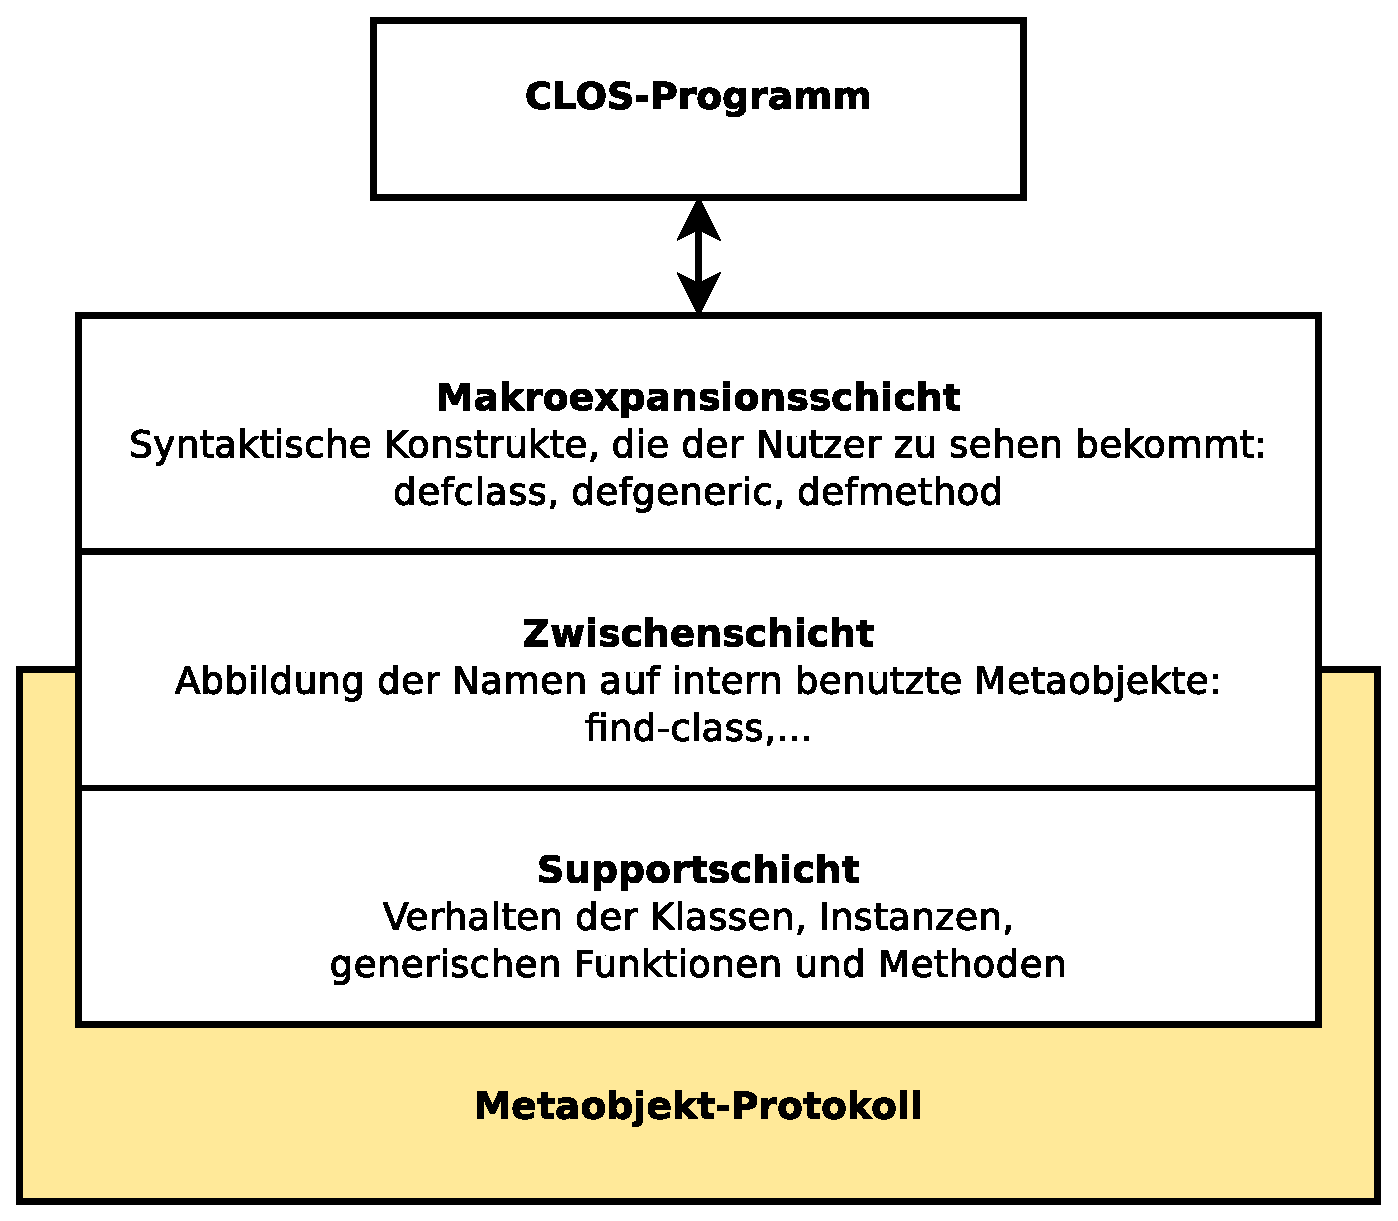
\includegraphics[width=0.65\textwidth]{pictures/mop}
  \caption{Struktur der CLOS-Implementierung nach AMOP}
 \end{figure}
\end{frame}

\begin{frame}
 \frametitle{Metaobjekte}
 \begin{itemize}
  \item \emph{Metaobjekte} = interne Objekte, die das Verhalten externer, dem Nutzer sichtbarer, Objekte beschreiben 
  \item für alle Konstrukte, die für den Benutzer definiert werden sollen und über die Informationen gesammelt werden müssen
  \begin{itemize}
   \item Klassenmetaobjekte
   \item Generische-Funktionen-Metaobjekte
   \item Methodenmetaobjekte
  \end{itemize}
  \item \emph{Metaklasse} = die Klasse, die das Verhalten von Metaobjekten definiert 
 \end{itemize}
\end{frame}

\begin{frame}[fragile]
 \frametitle{Klassenmetaobjekte}
 Ein Klassenmetaobjekt hält Informationen zu einer Klasse fest:
 \begin{itemize}
  \item Name
  \item direkte Superklassen
  \item direkte Slots
  \item Klassenpräzedenzliste
  \item effektive Slots
  \item direkte Subklassen
  \item direkte Methoden
 \end{itemize}
\end{frame}

\begin{frame}
 \frametitle{Von \texttt{defclass} zum Metaobjekt}
 \begin{itemize}
  \item \texttt{defclass}-Makro parst die Klassendefinition und verwandelt sie in einen Aufruf an die Funktion \texttt{ensure-class} aus der Zwischenschicht
  \item \texttt{ensure-class} erhält den Namen und die Argumente der Klasse und definiert ein benanntes Klassenobjekt
  \item Klassenmetaobjekte werden in einer Hashtabelle gespeichert
 \end{itemize}
 \vspace{0.5cm}
Es gibt drei Informationen, die sich nicht direkt aus der Klassendefinition ableiten lassen:
 \begin{itemize}
  \item Klassenpräzedenzliste
  \item geerbte Slots
  \item geerbte Methoden
 \end{itemize}
\end{frame}

\begin{frame}
 \frametitle{Klassenpräzedenzliste}
 \begin{itemize}
  \item beinhaltet die Klasse selbst und ihre Superklassen
  \item ohne Duplikate
  \item sortiert von spezifischster zu am wenigsten spezifischen Klasse
 \end{itemize}
 \vspace{0.5cm}
 Zwei Regeln bestimmen die Klassenpräzedenz:
\begin{enumerate}
 \item Eine Klasse hat immer Präzedenz über ihre Superklassen.
 \item Jede Klassendefinition legt die Präzedenzreihenfolge der direkten Superklassen fest.
\end{enumerate}
 \vspace{0.5cm}
 \begin{itemize}
  \item[\textbf{\textrightarrow}] CLOS wendet beide Definitionen rekursiv auf die Superklassenliste an, um die Klassenpräzedenzliste zu erhalten.
  \item anhand der KPL werden die effektiven Slots berechnet
 \end{itemize}
\end{frame}

\begin{frame}[fragile]
 \frametitle{Mehrfachvererbung und Methodenkombination}
 \begin{itemize}
  \item analog zu Klassen gibt es auch für Methoden und generische Funktionen Metaobjekte
  \item eine generische Funktion fasst eine Menge von implementierenden Methoden zusammen
 \end{itemize}
 \vspace{0.5cm}
 Generische-Funktionen-Metaobjekte merken sich:
 \begin{itemize}
  \item Name der Funktion
  \item Parameterliste
  \item implementierende Methoden
 \end{itemize}

\end{frame}

\begin{frame}[fragile]
 \frametitle{Mehrfachvererbung und Methodenkombination}
 \begin{itemize}
  \item Makros \texttt{defgeneric} und \texttt{defmethod} expandieren, analog zu \texttt{defclass}, zu einem Aufruf von \texttt{ensure-generic-function} bzw. \texttt{ensure-method}
  \item \texttt{ensure-generic-function} fügt eine neue generische Funktion zur Liste hinzu
  \item \texttt{ensure-method} fügt eine Methode zu einer generischen Funktion hinzu
  \item gibt der Benutzer nichts anderes an, wird die \textit{standard method combination} ausgeführt
 \end{itemize}
\end{frame}

\begin{frame}
 \frametitle{Methodenkombination}
 \begin{center}
  \begin{table}[h]\small
\begin{tabular}{|p{2.8cm}|p{3.3cm}|p{3.6cm}|}
 \hline
 \textbf{Schritt} & \textbf{Ergänzungsmethoden} & \textbf{Methodenkombination}\\\hline
 Bestimmen, welche Methoden anwendbar sind & Primärmethoden und Ergänzungsmethoden & Primärmethoden \\\hline
 Sortieren der anwendbaren Methoden nach Präzedenz & Sortieren der Methoden in der Reihenfolge Around, Before, spezifischste Primärmethode, After und innerhalb einer Kategorie nach Klassenpräzedenz & Sortieren der Methoden nach Klassenpräzedenz\\\hline
 Ausführen der Liste anwendbarer Methoden & Sequentiell & Kombination\\\hline
\end{tabular}
 \caption{Vorgehensweise bei der Methodenkombination.}
 \label{combination}
\end{table}
 \end{center}
\end{frame}

\section{Umsetzung}
\frame{\tableofcontents[currentsection]}

\begin{frame}
 \frametitle{Idee}
 \begin{itemize}
  \item grundsätzlich gleiches Vorgehen wie in CLOS
  \item Racketmetaobjekte anstatt CLOS-Metaobjekten
  \item Erzeugung von Objekten, Feldern und Methoden weiterhin Racket überlassen
  \item Syntax der Klassenerzeugung geschickt manipulieren
  \item damit Mehrfachvererbung erreichen
 \end{itemize}
 \vspace{0.5cm}
 Im Rahmen dieser Arbeit ist ein Protoyp für eine solche Erweiterung entstanden.\\
 \textbf{\textrightarrow} Probleme, die bei der Implementierung auftraten und wie sie gelöst wurden
\end{frame}

\begin{frame}
 \frametitle{Benannte Klassen}
 \textbf{Problem:} Klassen in Racket sind nicht benannt
 \vspace{0.5cm}
 \begin{itemize}
  \item[\textbf{\textrightarrow}] erzeugtes Klassenobjekt als Schlüssel
  \item[\textbf{\textrightarrow}] Metaobjekt kann erst \texttt{nach} Erzeugung des eigentlichen Klassenobjekts in die Tabelle eingefügt werden
 \end{itemize}
\end{frame}


\begin{frame}
 \frametitle{Keine Feld- und Methodenobjekte}
 \textbf{Problem:} Nicht möglich Feld- und Methodenobjekte zu erzeugen.
 \vspace{0.5cm}
 \begin{itemize}
  \item kein Zugriff 
  \item[\textbf{\textrightarrow}] anstelle der Objekte wird die Definition der Felder/Methoden festgehalten
 \end{itemize}
\end{frame}

\begin{frame}
 \frametitle{Mehrfachvererbung und Ergänzungsmethoden}
 \textbf{Problem:} Darstellung von Ergänzungsmethoden ist schwierig.
 \vspace{0.5cm}
 \begin{itemize}
  \item Kennen nur die Definition der Methoden
  \item Wie mit Aufrufen von \texttt{super} oder \texttt{inner} umgehen?
  \item Auswirkung auf Methodenkombination?
  \item[\textbf{\textrightarrow}] Workaround für den Protoyp: Ergänzungsmethoden bei Mehrfachvererbung ignorieren
  \item[\textbf{\textrightarrow}] nur mit \texttt{define/public} definierte Funktionen werden (mehrfach-) vererbt und gehen in die Kombination ein
 \end{itemize}
\end{frame}

\begin{frame}
 \frametitle{Mehrere Superklassen}
 \textbf{Problem:} Racket erlaubt es nicht, mehrere Superklassen anzugeben
 \vspace{0.5cm}
 \begin{itemize}
  \item Racket übernimmt am Ende Objekterzeugung 
  \item Klassendfinition darf nur eine Superklasse enthalten
  \item[\textbf{\textrightarrow}] Erzeuge eine Klasse, welche die Eigenschaften aller ursprünglichen Superklassen vereinigt
  \item[\textbf{\textrightarrow}] übergebe diese als offizielle Superklasse
 \end{itemize}
\end{frame}

\begin{frame}
 \frametitle{Methodenkombination}
  \textbf{Problem:} Racket erlaubt keine Redeklaration von Methoden.
   \vspace{0.5cm}
  \begin{itemize}
   \item Methodenkombination nicht sehr effektiv, wenn es nur eine Methode gibt
   \item[\textbf{\textrightarrow}] Redeklaration von mit \texttt{define/public} deklarierten Methoden erlauben, wenn an MK beteiligt
   \item Methoden vor der Erzeugung der Klassenobjektes wieder entfernen
   \item auch aus Superklassen
   \item Original-Superklassen können nicht weiterverwendet werden
   \item[\textbf{\textrightarrow}] auch hier eigens erstellte Superklasse verwenden
  \end{itemize}
\end{frame}

\begin{frame}
 \frametitle{Methodenkombination und geerbte Felder}
 \textbf{Problem:} Geerbte Eigenschaften innerhalb der Klassendefinition nur sichtbar, wenn mit \texttt{inherit} / \texttt{inherit-field} deklariert
 \vspace{0.5cm}
 \begin{itemize}
  \item ggf. für Methodenkombination benötigt
  \item in der Subklasse nicht ohne weiteres sichtbar
  \item eine Möglichkeit: automatisch für alle Felder eine \texttt{inherit-field}-Option einfügen, wenn Methodenkombination beteiligt
  \item kann zu Verwirrung führen, wenn manchmal \texttt{inherit-field} angegeben werden muss und manchmal nicht
  \item[\textbf{\textrightarrow}] Nutzer muss per Hand dafür sorgen, dass benötigte Felder sichtbar sind
 \end{itemize}
\end{frame}

\begin{frame}
 \frametitle{\texttt{define/generic}}
 \textbf{Problem:} Racket kennt keine \texttt{define/generic} Option
 \vspace{0.5cm}
 \begin{itemize}
  \item[\textbf{\textrightarrow}] muss vor der Erzeugung des Klassenobjekts aus der Liste der Klassenoptionen entfernt werden
 \end{itemize}
\end{frame}

\begin{frame}
 \frametitle{\texttt{eval} im Definitionsfenster}
 \textbf{Problem:} Auswerten der erstellten Klassendefinition
 \vspace{0.5cm}
 \begin{itemize}
  \item selbst zusammengebaute Klassendefinition muss ausgewertet werden, um ein Klassenobjekt zu erhalten
  \item \texttt{eval} tut genau das
  \item funktioniert ohne weiteres nur im Interaktionsfenster
  \item \texttt{eval} benötigt einen Kontext
  \item[\textbf{\textrightarrow}] ``Zwischenexpansion'', in der der lokale Kontext in einem Namensraum festgehalten wird
  \item[\textbf{\textrightarrow}] Namensraum mit an das eigentliche Makro übergeben
 \end{itemize}
\end{frame}

\section{Fazit}
\frame{\tableofcontents[currentsection]}

\begin{frame}
\frametitle{Auswertung}
 \begin{itemize}
  \item es ist möglich, das Pokemon-Beispiel im Protyp zu definieren
  \item sehr einfach, CLOS-ähnlich
  \item Ergänzungsmethoden werden noch nicht unterstützt
  \item Prototyp hat einige Einschränkungen
  \item eignet sich jedoch bereits für die Verwendung in der Lehre
  \item eignet sich für Projekte, in denen Methoden hauptsächlich mit \texttt{define/public} definiert werden
 \end{itemize}
\end{frame}

\begin{frame}
 \frametitle{Einschränkungen}
 \begin{itemize}
  \item nur \texttt{field}, \texttt{init-field}, \texttt{define/public} unterstützt
  \item direkte Superklasse der neuen Superklasse ist \texttt{object\%}
  \item Methoden, die an Methodenkombination beteiligt sind, 
  \begin{itemize}
   \item können beliebig mit \texttt{define/public} redeklariert werden
   \item sind in der Superklasse anschließend nicht mehr vorhanden
  \end{itemize}
  \item \texttt{inherit-field} ggf. notwendig
  \item Namen für generische Funktionen müssen eindeutig sein
  \item Kombinationsmethoden werden am Ende der Klassendefinition eingefügt (nach \texttt{super-new})
  \item Methodenkombination nicht kompatibel mit Ergänzungsmethoden
  \end{itemize}
\end{frame}

\begin{frame}
 \frametitle{Fazit}
 \begin{itemize}
  \item mithilfe von Makros und dem Metaobjektprotokoll Prototyp für Mehrfachvererbung in Racket implementiert
  \item im Entwurf formulierte Anforderungen erfüllt
  \item deutlich unterschiedliches Objektsystems 
  \item nur geringfügige Anpassungen notwendig
  \item Quelltext ist sehr kompakt
   \end{itemize}
  \end{frame}
  
\begin{frame}  
 \frametitle{Fazit}
  \begin{itemize}
  \item Beschränkung auf Teilmenge der Klassenoptionen von Racket
  \item Erweiterung um andere (oder gar alle) Klassenoptionen würde Metaobjekte und Bestimmung der zu vererbenden Eigenschaften deutlich komplexer machen
  \item bei Pokemonbeispiel kein Unterschied in der Effizienz messbar
  \item kann bei größeren Projekten anders sein
 \end{itemize}
\end{frame}

\begin{frame}
 \frametitle{Fazit}
 \begin{center}
 Insgesamt lässt sich sagen:\\
 \vspace{1cm}
 \textbf{Das Metaobjektprotokoll eignet sich zur Erweiterung eines bestehenden Objektsystems.}
 \end{center}
\end{frame}

% \begin{frame}
%  \frametitle{Ausblick}
%  Erweiterungsvorschläge:
%  \begin{itemize}
%  \item Ergänzungsmethoden implementieren
%  \item Ermitteln, welche Klassenoptionen mit der Erweiterung kompatibel sind und welche nicht
%  \item Evaluieren, welche anderen Klassenoptionen sich für Mehrfachvererbung eignen und diese implementieren
%  \item Die Effizienz verbessern
%  \item Die Erweiterung im Übungsbetrieb von ``Softwareentwicklung III'' testen
%  \item Veranlassen, dass in einer neueren Racketversion \texttt{compute-std-cpl} exportiert wird, damit der Quelltext nicht kopiert werden muss
%  \item Veranlassen, dass die Erweiterung zu einer zukünftigen Version von Racket hinzugefügt wird 
% \end{itemize}
% \end{frame}

\begin{frame}
\begin{center}
  Danke für die Aufmerksamkeit!
\end{center}
\end{frame}
\end{document}